% !TEX root = ../thesis.tex

\chapter{Syntactic part}
\label{sec:methodology}
\section{Goal of the work} \label{sec:goal}
Based on the analytical part~\ref{sec:analytical} I will be working on a mathematical model to predict customer behavior consist of vendor,
psychology and loyalty sub-models combine in hidden markov model (HMM) to final prediction model.
States in the HMM will be read by viterbi algoritm~\ref{subsec:viterbi} which is able to predict most probability state in propagation by HMM.
I try to get a better results than actual standard statistic method (Time Series analysis) to predict customer behavior in e-commerce.
\section{Modeling prediction of customer behavior} \label{sec:modeling}
The goal of model is to predict probability that customer will successfully finish order. This model will be consist of three submodels.
Vendor model,\ psychology model and loyalty model. All sub-models will be combine to complex prediction mechanism, as you can see on image~\ref{Model schema with interaction}
To final prediction will be used Hidden Markov model in combination with Viterbi algorithm to detect hidden states to reflect set weights and get better results for each industry.
\\
\begin{figure}[h!]
    \begin{center}
        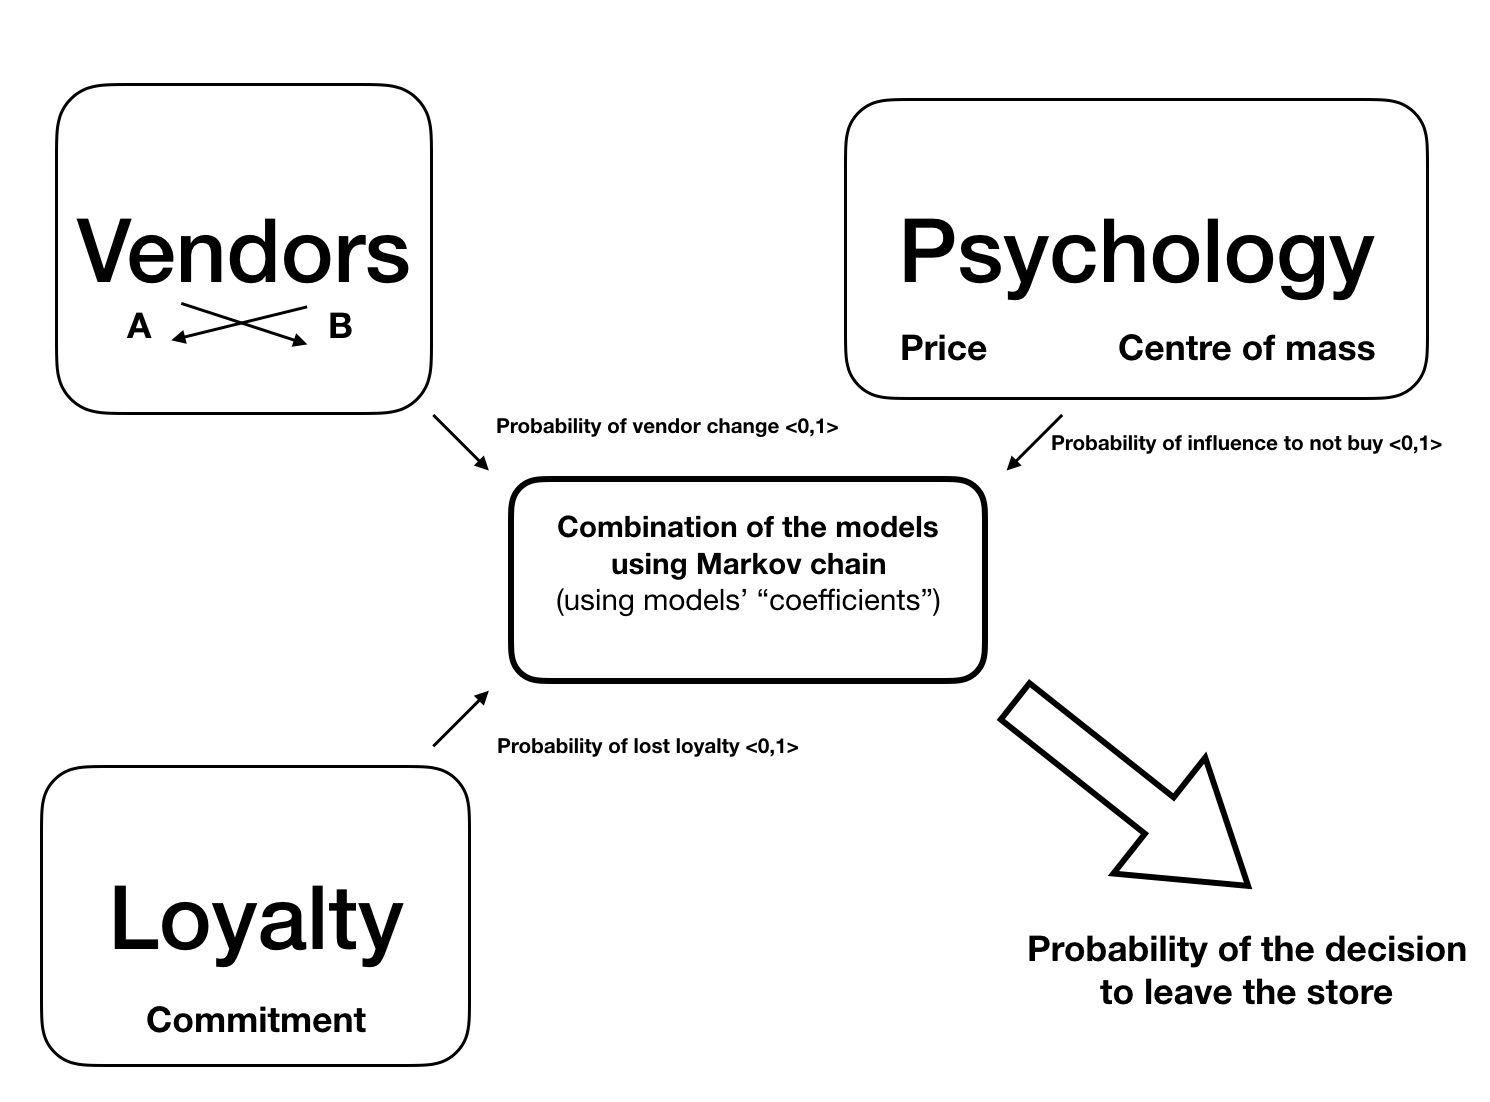
\includegraphics[width=140mm]{computation_schema.png}
    \end{center}
    \caption{Computation flow and interactions between models}
    \label{Model schema with interaction}
\end{figure}
\\
\subsection{Preprocessing of input data} \label{subsec:preprocessing}
Data should have to be anonymized \footnote{Data anonymization is a type of information sanitization whose intent
is privacy protection.
It is the process of either encrypting or removing personally identifiable information from data sets, so that
the people whom the data describe remain anonymous.} and pseudonymized \footnote{Pseudonymization is a data management
and de-identification procedure by which personally identifiable information fields within a data record are replaced
by one or more artificial identifiers, or pseudonyms.} to keep legal notice of~\cite{gdpr}.
Than we should utilized data to utilized inputs.
Prepared data will be stored as csv files and than will be imported to Matlab for computation.
\newpage
\subsection{Vendors} \label{subsec:model_vendors}
For simplification we will take to account only a two vendors market share, without 100\% domination, because of on a real
market is 100\% monopole unlikely see and than we will be reflect only main competitor.
From that condition it will see that for market dominate vendor it will return false positive results.
Our model is based on equations from Brands section~\ref{eq:10} and from those equation we will get probability of vendor change from
vendor $A$ to vendor $B$ and if the vendor $B$ will have more strength than vendor $A$ it will break the computation and customer
will leave our store without successfully completing buy process.
Results of this computation wil be probability for each iteration of buy process simulation in an interval $<0,1>$. Data for this model
will comes from open data from google.com, heureka.cz/heureka.sk and national governments.
\\
\begin{equation} \label{eq:24}
\alpha_{xy} = \beta H(P_x-P_y) + \gamma H(Qx-Qy) + \delta H(Px-Py)H(Q_x - Q_y)
\end{equation}
\\
where $\beta, \gamma, \delta$ are non-negative.
\\
\begin{itemize}
    \item $P$ is prices of vendors products
    \item $Q$ is a quality index of vendor
    \item $H$ is a Heaviside function which will be calculated by~\ref{eq:22}.
\end{itemize}
\\
\begin{eqnarray} \label{eq:25}
H(s) = 1, s > 0 \\
H (s) = 0, s \leq 0
\end{eqnarray}
\\
\subsection{Psychology} \label{subsec:model_psychology}
Psychology aspect is trying to simulate customer behavior in thee situation like a prices aspect, society influenced, mood aspect, actual needs
and so on.
In this model we will simplify only for price effect~\ref{subsubsec:model_psychology_price} and center of mass effect~\ref{subsubsec:model_psychology_mass}
\subsubsection{Price aspect} \label{subsubsec:model_psychology_price}
\begin{equation} \label{eq:26}
\overset{-}{Q} = \frac{1}{n_p} \sum_{i=1}^{n_p} Q_i
\end{equation}
\\
\begin{itemize}
    \item $Q_i$ number of orders for product $i$ per day divide amount of orders per same day, prom interval $<0,1>$
    \item $n_p$ number of products in store
\end{itemize}
\\
\begin{equation} \label{eq:27}
\alpha_{ij} = \frac{C+d(Q_j, \overset{-}{Q})}{C+d(Q_i, \overset{-}{Q})}
\end{equation}
\\
Coefficient C is used to be $\alpha_{ij}$ always positive.
\subsubsection{Center of mass aspect} \label{subsubsec:model_psychology_mass}
Center of mass aspect is applied as a part of sociology to our psyhology.
Marketers use it to manipulate with customers in global way.
Like a black friday, Cyber monday etc., in that days stores manipulate with our psychology by discount prices.
\\
\begin{equation} \label{eq:28}
\overset{-}{P} = \frac{1}{n_p} \sum_{i=1}^{n_p} P_i
\end{equation}
\begin{itemize}
    \item $P_i$ is defined as product price minus retail recommend price divide average price
    \item $n_p$ number of products in store
\end{itemize}
\\
\begin{equation} \label{eq:29}
\alpha_{ij} = \frac{C+d(P_j, \overset{-}{P})}{C+d(P_i, \overset{-}{P})}
\end{equation}
\\
This model return probability for customer decision to make action from interval $<0,1>$.
\\
\subsection{Loyalty} \label{subsec:model_loyalty}
This models is based on Luarn & Lin research~\cite{luarn} and change it's model for our needs.
\begin{equation} \label{eq:30}
L = \frac{R+Z}{Z}
\end{equation}
\\
\begin{enumerate}
    \item L ..... probability of whole loyalty model
    \item R ..... probability of separate loyalty model
    \item Z ..... probability of commitment model
\end{enumerate}
\\
As we see on~\ref{Loyalty scheme} Loyalty model is consist of all three sub-models (Trust, Customer Satisfaction, Perceived value)
but commitment model consist of only Trust and Customer Satisfaction.
a,b,c,d,e .... weight coefficient to combine Trust, Customer satisfaction and Perceived value.

Trust
\begin{equation} \label{eq:31}
T = \frac{1}{n} \sum_{i=1}^{n} O_i
\end{equation}

$O_i$ number of orders divide number of visitors per day $i$

\textbf{Customer satisfaction} are datasets get from open data per each day, individual satisfaction.
For this situation will be simplified to average satisfaction per whole store.
\textbf{Perceived value} is subjective value, which depends of strength of the store, data will be get from vendor model.
\subsubsection{Commitment} \label{subsubsec:model_loyalty_commitment}
\textbf{Commitment} is making the actual choice everyday or other period basis to keep up with something e.g. a relationship, personal goal, a task, etc.
You would have to hold yourself accountable to keep a commitment to something or someone.
Similarly, being loyal involves holding yourself accountable as well.
Against of \textbf{Loyalty} which is is usually seen as a character trait rather than a conscious decision.\\
This model return probability for customer decision to not leave the store from interval $<0,1>$.

\begin{figure}[h!]
    \begin{center}
        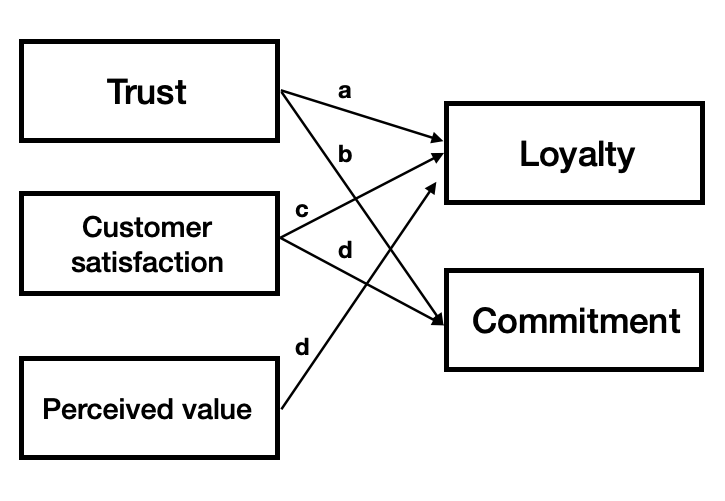
\includegraphics[width=140mm]{loyalty.png}
    \end{center}
    \caption{Computation flow for loyalty and commitment}
    \label{Loyalty scheme}
\end{figure}
\subsection{Combining models to decision process} \label{subsec:combining_models}
All separates models return probabilities vectors which we use as input to Hidden Markov model (HMM) \footnote{Hidden Markov Model (HMM) is a statistical Markov model
in which the system being modeled is assumed to be a Markov process with unobservable (i.e. hidden) states.
The hidden Markov model can be represented as the simplest dynamic Bayesian network.
The mathematics behind the HMM were developed by L. E. Baum and coworkers.
HMM is closely related to earlier work on the optimal nonlinear filtering problem by Ruslan L. Stratonovich,
who was the first to describe the forward-backward procedure.}
These probabilities will be combine with specific weights coefficients to prevent always positives results.
\section{Prediction application} \label{sec:app}
Application will import previous data about visitors and earn of project in csv format, in admin part is able to
create industry for setting wages to each one, than return graph results for prediction based on imported data,
industry setting and time period.

\section{Decision process from submodels} \label{sec:decision}
\subsection{Hidden markov model} \label{subsec:hhm}
In a Hidden Markov Model (HMM), we have an invisible Markov chain (which we cannot observe), and each state
generates in random one out of k observations, which are visible to us. Let’s look at an example.
Suppose we have the Markov Chain from above, with three states (snow, rain and sunshine),
P - the transition probability matrix and q — the initial probabilities.
This is the invisible Markov Chain — suppose we are home and cannot see the weather.
We can, however, feel the temperature inside our room, and suppose there are two possible observations: hot and cold.
(TODO Write a mechanism and equation to combine models to final probabilty)
\subsection{Used software and libraries} \label{subsec:libraries}
\begin{enumerate}
    \item Matlab 2019b
    \item ReGUI builder
\end{enumerate}
\section{Decision algoritm}
\subsection{Flowcharts}
\subsubsection{Overview}
\begin{figure}[h!]
    \begin{center}
        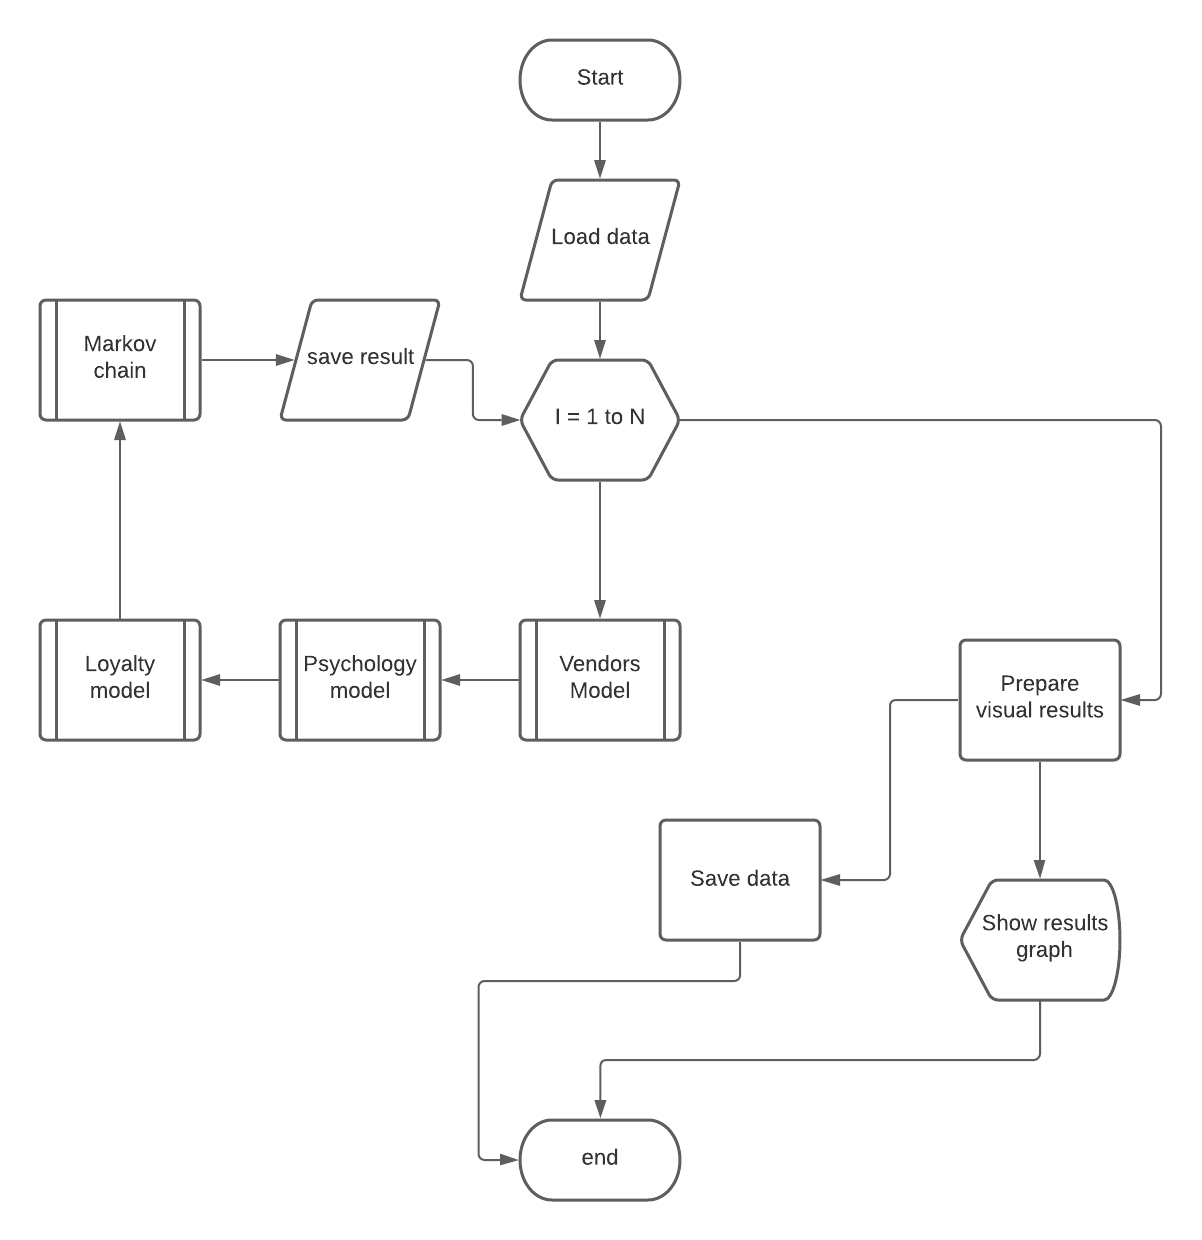
\includegraphics[width=350]{flowchart_overview}
    \end{center}
    \caption{Flowchart overview}
    \label{flowchart_overview}
\end{figure}
\newpage
\subsubsection{Vendor model}
\begin{figure}[h!]
    \begin{center}
        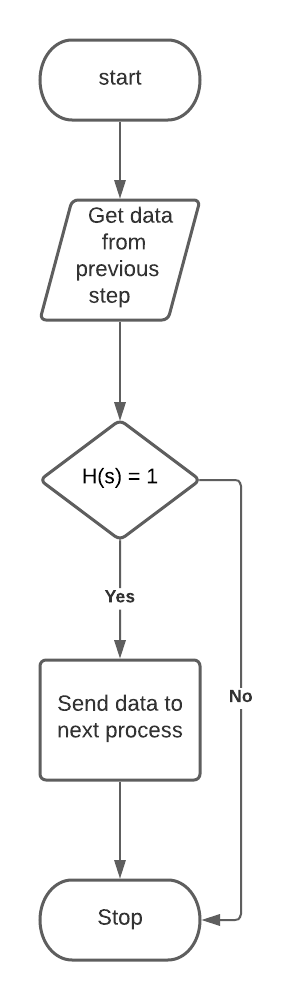
\includegraphics[width=180]{flowchart_vendor}
    \end{center}
    \caption{Flowchart vendor model}
    \label{flowchart_vendor}
\end{figure}
\subsubsection{Psychology model}
\begin{figure}[h!]
    \begin{center}
        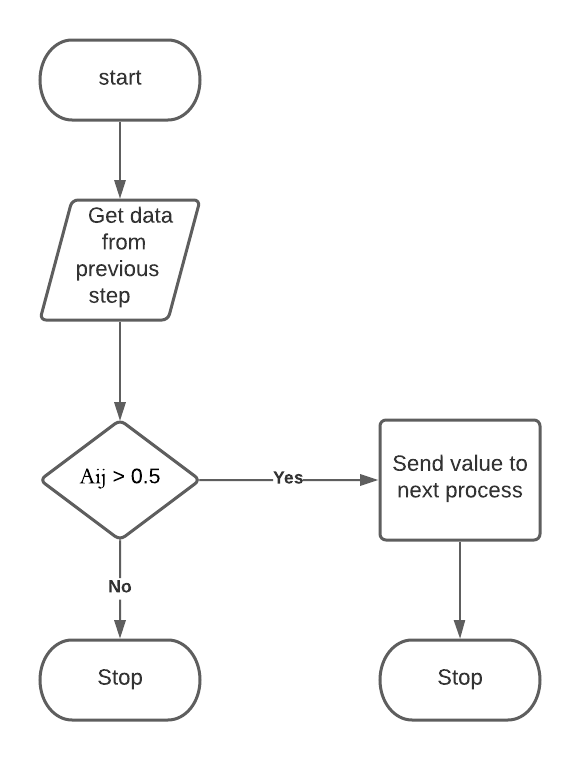
\includegraphics[width=180]{flowchart_psychology}
    \end{center}
    \caption{Flowchart psychology model}
    \label{flowchart_psychology}
\end{figure}
\newpage
\subsubsection{Loyalty model}
\begin{figure}[h!]
    \begin{center}
        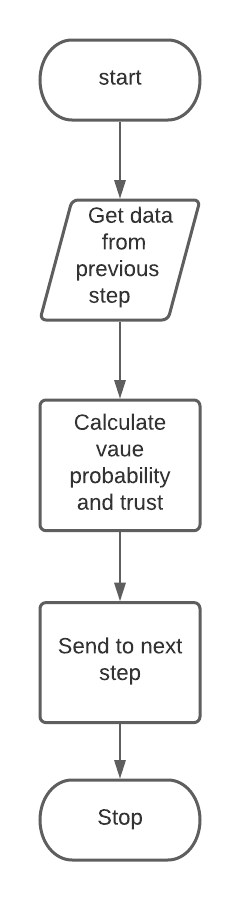
\includegraphics[width=60]{flowchart_loyalty}
    \end{center}
    \caption{Flowchart loyalty model}
    \label{flowchart_loyalty}
\end{figure}
\subsubsection{Markov hidden model}
\begin{figure}[h!]
    \begin{center}
        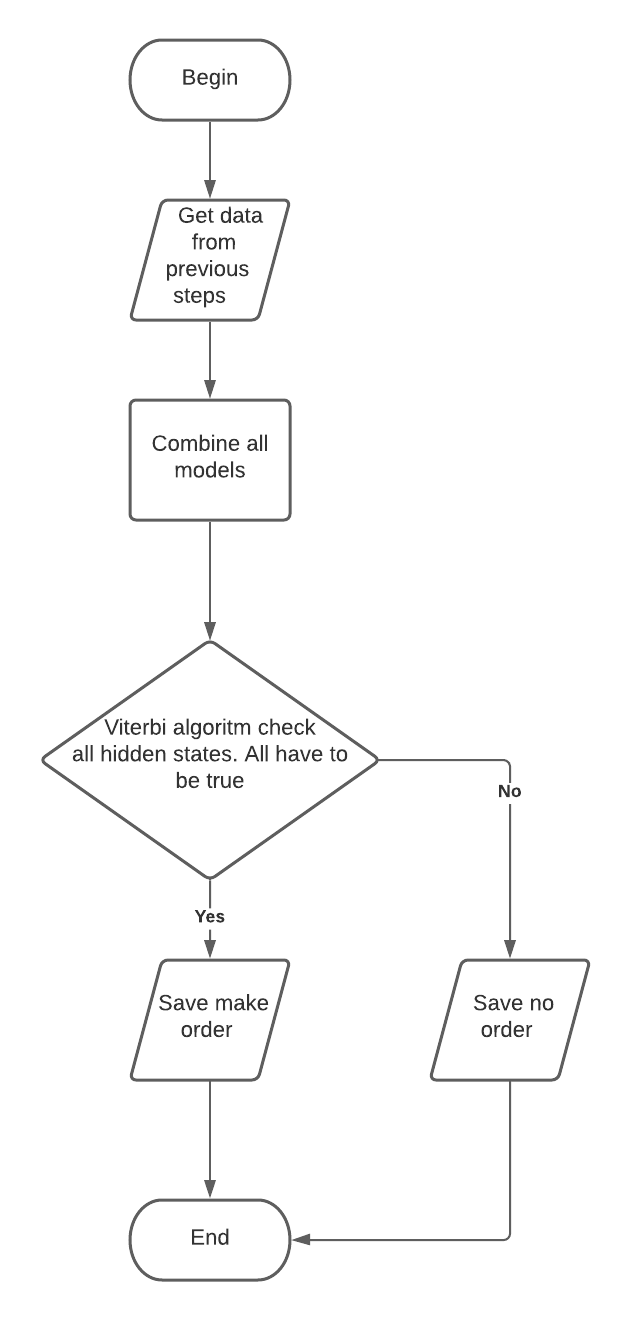
\includegraphics[width=230]{flowchart_markovpng}
    \end{center}
    \caption{Flowchart markov chain}
    \label{flowchart_markov}
\end{figure}
\newpage
\subsection{Time series}
\subsubsection{Moving average}
As a first basic time series analysis we tried moving averages. These method looks like not usefull for our needs,
because of not reflecting trend in e-commerce. Specific e-commerce trends as Christmas time and new years discounts.
\begin{figure}[h!]
    \begin{center}
        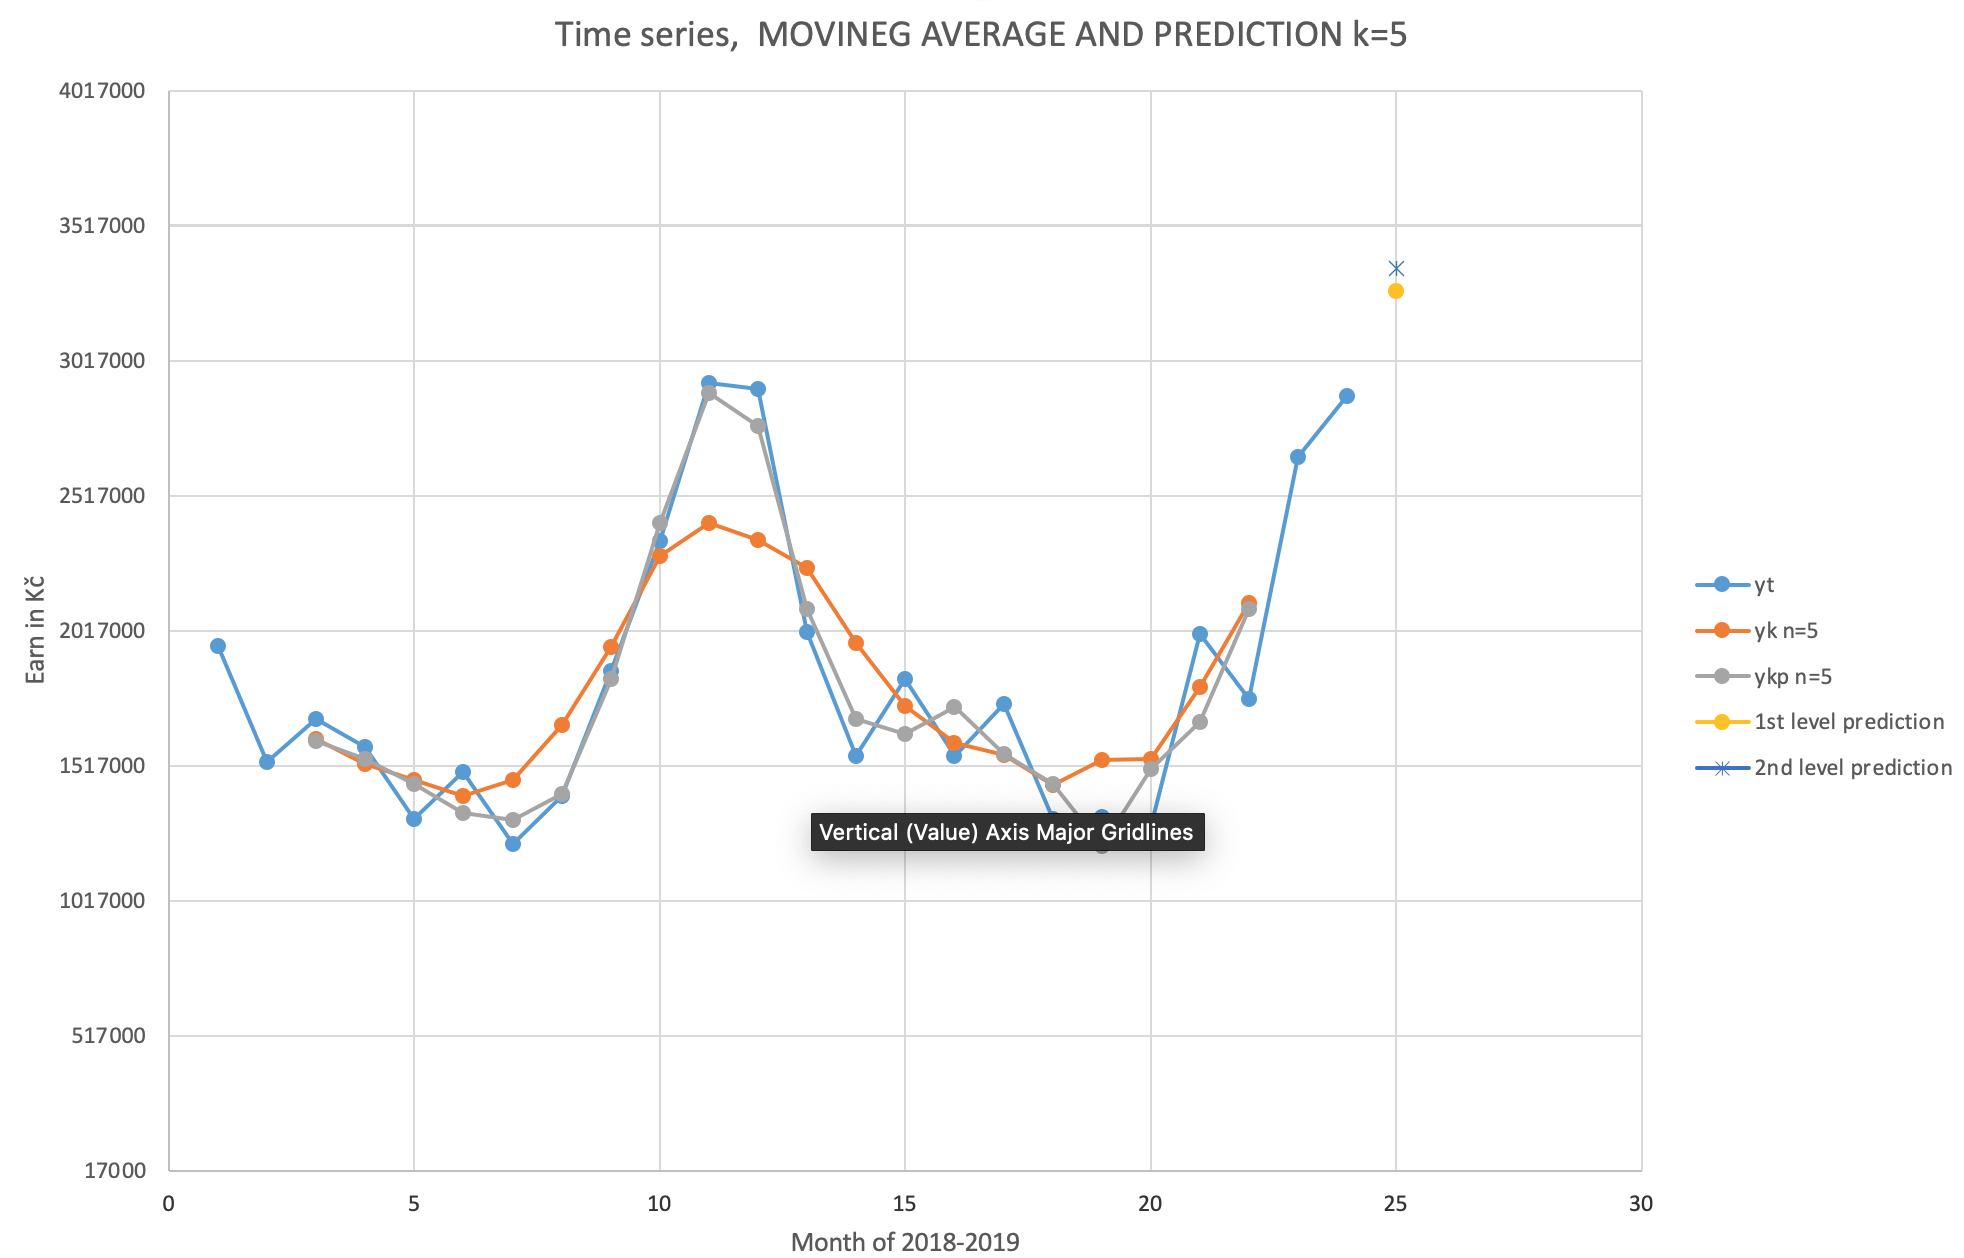
\includegraphics[width=140mm]{moving_average.png}
    \end{center}
    \caption{Moving average results}
    \label{Time series moving average}
\end{figure}
\newpage
\subsubsection{Models}
More better results we get from model $Tr_{t2}=a_0+a_1t+a_2t^2$. But the goal is not to find the best
statistics solution in time series, so this model is enough as a reference. Time series analysis get the
result of 14,56\% aberrance from the real 2020 data.
\begin{figure}[h!]
    \begin{center}
        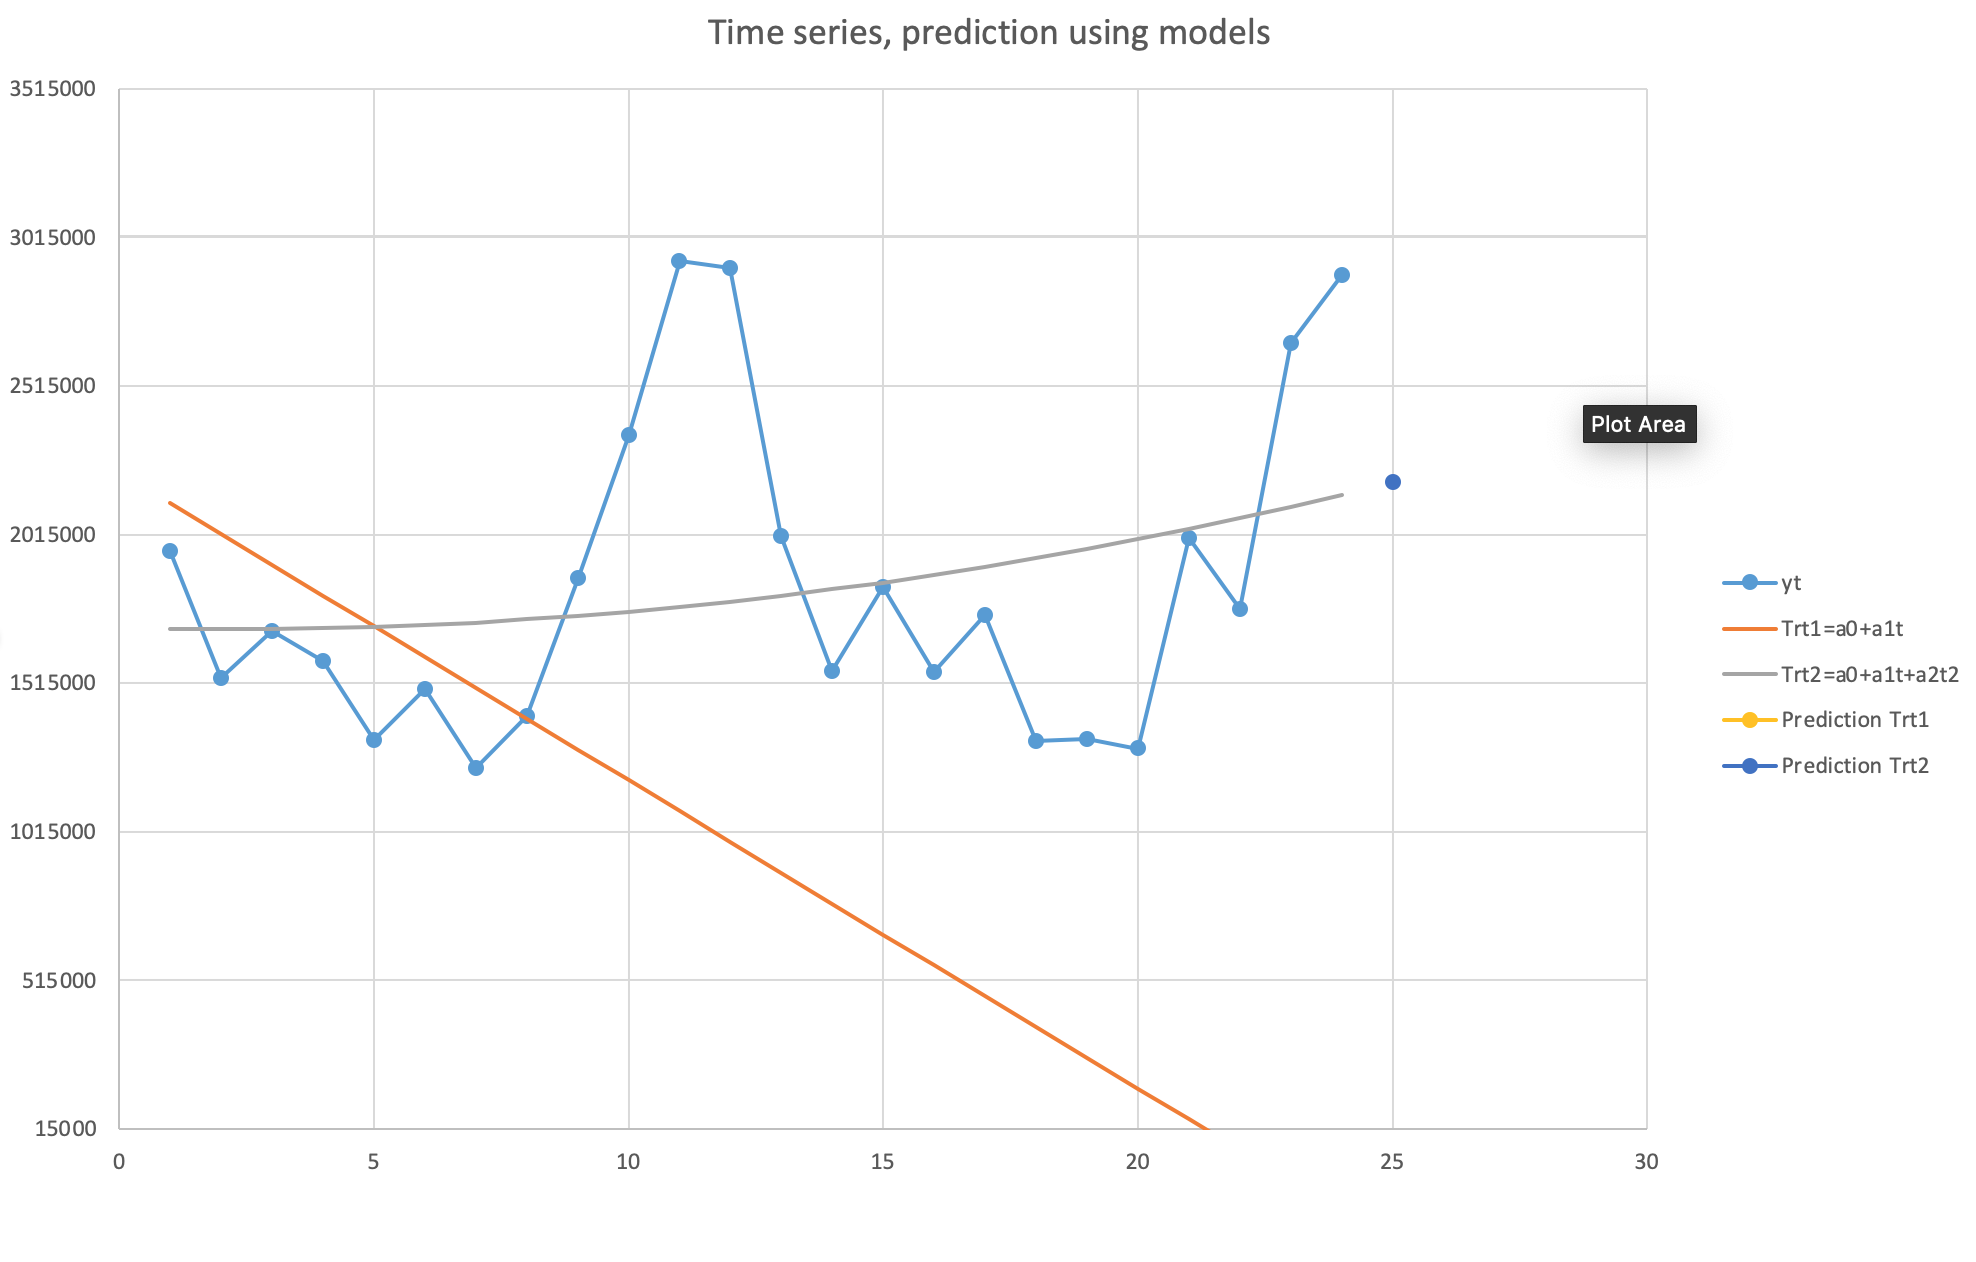
\includegraphics[width=140mm]{model_ts.png}
    \end{center}
    \caption{Time series model results}
    \label{Time series model's}
\end{figure}
